\section{Transformers}

It is impossible to discuss Transformers without referring to the seminal work "Attention is All You Need" \cite{vaswani2023attention}.\\

The Transformer architecture, proposed by Vaswani et al., revolutionized the field of natural language processing by introducing a model that relies entirely on attention mechanisms, dispensing with recurrence and convolutions. This shift allowed for more parallelization and significant improvements in computational efficiency.\\

The Transformer model is composed of an encoder and a decoder, each of which is a stack of identical layers. The primary innovation is the self-attention mechanism, which allows the model to weigh the importance of different vectors in the input sequence when producing an output. \\

The self-attention mechanism is complemented by positional encoding, which injects information about the relative or absolute position of the tokens in the sequence. This is crucial because, unlike recurrent neural networks, Transformers do not inherently capture the order of the input sequence.\\

In addition to self-attention, each layer in the Transformer includes a feed-forward neural network and normalization steps. Residual connections are employed around each sub-layer, followed by layer normalization, which helps to stabilize the learning process.\\

Let us look at this figure which was found in the paper by Vaswani et al.:\\

\begin{figure}[ht]
    \centering
    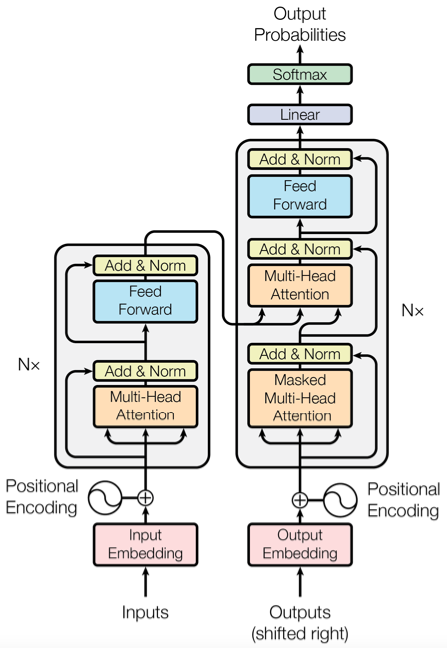
\includegraphics[width=0.4\textwidth]{media/Architecture_transfo.png}
    \caption{architecture of a transformer}
    \label{fig:transfo}
\end{figure}

\subsection{ViT}

ViT, or Vision Transformer, is a type of Transformer model that has been adapted for computer vision tasks \cite{dosovitskiy2021image}. \\

In the ViT model, an image is split into fixed-size patches, which are then linearly embedded. The resulting vectors serve as the input to the Transformer, similar to how word embeddings are used in NLP tasks. The key insight is that the self-attention mechanism can be used to model relationships between these image patches, much like it models relationships between words in a sentence.\\

The ViT model also uses positional embeddings to retain spatial information about the patches, similar to how positional encoding is used in the original Transformer. The output of the Transformer is then passed through a linear layer to produce the final image classification.\\

The ViT model has been shown to perform competitively with state-of-the-art convolutional neural networks on various image classification benchmarks. This demonstrates the versatility of the Transformer architecture and suggests that it could be a promising direction for future research in computer vision.\\

\subsection{Swin Transformer}

The Swin Transformer, introduced by Liu et al. \cite{liu2021swin}, is a hierarchical Transformer whose representation is computed using shifted windows. This model aims to address the issue of quadratic complexity with respect to the image size in standard Transformers by limiting self-attention computation to non-overlapping local windows. The shifted window approach allows for cross-window connections, enabling the modeling of long-range dependencies while maintaining computational efficiency.\\

\subsection{U-Transformer}

The U-Transformer is a variation of the Swin Transformer and is constructed using 48 repeated Swin Transformer V2 blocks. This model leverages the strengths of the Swin Transformer, such as its ability to model long-range dependencies efficiently, and combines them with a U-Net like architecture to provide a powerful tool for tasks requiring detailed, high-resolution output, such as semantic segmentation.\\
